\chapter{Teoría de la Computabilidad}\label{ch:teoria-de-la-computabilidad}
Clasificar los distintos problemas y formalizar el concepto de computar.

$\left\{\begin{matrix}
    Complejidad& \left\{\begin{matrix}
    Algoritmo &\rightarrow& \textit{Coste temporal } T(n)\\ 
    Problemas &\rightarrow& \textit{Tipo de problema según complejidad} \left\{\begin{matrix}
    P\\ 
    NP\\ 
    NPC
    \end{matrix}\right.
    \end{matrix}\right.\\ 
    Computabilidad& \rightarrow Problema \left\{\begin{matrix}
    Computable\\ 
    \textit{No computable}
    \end{matrix}\right.
    \end{matrix}\right.$

\textbf{Problema:} Descripción de una pregunta que requiere una respuesta.
\begin{itemize}
    \item p: instancia $\rightarrow$ respuesta
    \item $x \rightarrow p(x)$
\end{itemize}

\textbf{Instancia:} Especificación exacta de los datos de un problema para un caso particular.

\textbf{Algoritmo:} Conjunto de instrucciones que garantiza encontrar una solución correcta para cualquier instancia en un \textbf{número finito de pasos}.

\textbf{Analogía geométrica:} Hallar el lado de un cuadrado inscrito en un círculo, se puede dibujar fácilmente, pero en cuanto a matemáticas nunca se halla exactamente al tener raíces cuadradas. $r^2 = \frac{l^2}{2}+\frac{l^2}{2}; \; l= \sqrt{2}r$. Un caso en el que no es posible de ambas manera es dibujar un cuadrado con la misma área que un círculo, dado que entra en juego $\sqrt{\pi}$. $l^2 = \pi r^2; \; l = \sqrt{\pi}r$

\section{Problema de Satisfabilidad Booleana: SAT}
Un problema SAT 2 puede describirse usando una expresión booleana con una forma restringida especial. Es una conjunción de cláusulas, donde cada \textbf{cláusula} es una disyunción de \textbf{dos variables}. Las variables o las negaciones de variables que aparecen en la fórmula se denominan literales.
\begin{itemize}
    \item $(x \vee z) \wedge (y \vee w) \wedge (\overline{y} \wedge z)$
\end{itemize}

if x then y else z

$(x \wedge y) \vee (\overline{x} \wedge z)$
\pagebreak

\subsection{Algoritmo sencillo}
Generar un conjunto de posibles asignaciones (permutaciones) para todas las entradas.
\begin{itemize}
    \item Evaluar el resultado de la expresión entera usando esta asignación
    \item Repetir hasta encontrar una solución
\end{itemize}
Es eficaz y eficiente para instancias pequeñas.

En cuanto a coste no hay un algoritmo conocido que garantice la solución de este problema en un tiempo polinómico en el número de variables.

\subsection{Aplicaciones}
Muchos Problemas de decisión se pueden reformular en términos del problema de Satisfacibilidad.
\begin{itemize}
    \item Verificación de HW / SW.
    \item Planning
    \item Constraint Programming
    \item Linear Programming
\end{itemize}

\section{Clique}
Un clique es un conjunto $C$ de vértices donde todo par de vértices de $C$ esta conectado con una arista en $G$, es decir un Clique $C$ es un subgrafo completo.

Subgrafo completo, en el que todos los vértices están conectados con todos.

Tiene mucha potencia social, todos conocen o comparten gustos.

\subsection{Aplicaciones}
\begin{itemize}
    \item Link farms
    \item Segmentación de imágenes y reconocimiento de patrones, reconocimiento de regiones
    \item Redes Bayesianas, cálculo de probabilidades condicionales.
    \item Biología, analizar proteínas similares
\end{itemize}

\section{Decidibilidad}
Un problema de computación puede considerarse como un lenguaje.

Las posibles soluciones del problema pueden considerarse como las palabras que pertenecen al lenguaje.
\begin{itemize}
    \item Ejem. $ax^2+bx+c=0$
    \item Problema: Tiene solución la ecuación en $\mathbb{R}$
    \item Respuestas $\in \{Si, No\}$
    \item Soluciones $\in \mathbb{R}$
    \item Lenguaje: $L= \{a,b,c\}$
\end{itemize}

\begin{figure}[H]
    \ffigbox[\FBwidth]
    {\caption{Diagrama Decidibilidad}}
    {\tikzset{every picture/.style={line width=0.75pt}}
    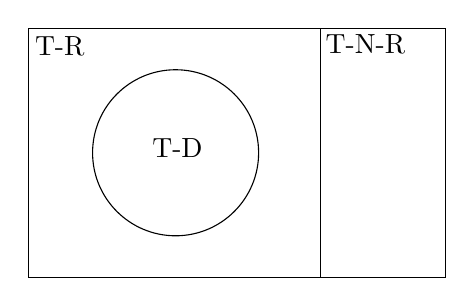
\begin{tikzpicture}[x=0.75pt,y=0.75pt,yscale=-1,xscale=1]
    \draw   (179,100) -- (380,100) -- (380,220) -- (179,220) -- cycle ;
    \draw   (210,160) .. controls (210,137.91) and (227.91,120) .. (250,120) .. controls (272.09,120) and (290,137.91) .. (290,160) .. controls (290,182.09) and (272.09,200) .. (250,200) .. controls (227.91,200) and (210,182.09) .. (210,160) -- cycle ;
    \draw    (320,100) -- (320,220) ;
    
    \draw (181,103) node [anchor=north west][inner sep=0.75pt]   [align=left] {T-R};
    \draw (321,102) node [anchor=north west][inner sep=0.75pt]   [align=left] {T-N-R};
    \draw (237.5,152) node [anchor=north west][inner sep=0.75pt]   [align=left] {T-D};
    \end{tikzpicture}}
\end{figure}
\begin{itemize}
    \item \textbf{T-D:} Turing-Decidible. Es un problema para el cual una MT acepta todas las soluciones y rechaza las que no son. \\ Se para siempre.
    \item \textbf{T-R:} Turing-Reconocible, pero no decidible. Es un problema para el cual la MT acepta todas las que son soluciones. \\ Puede entrar en bucle para las no soluciones.
    \item \textbf{T-N-R:} Turing-No-Reconocible. Ni acepta las que son soluciones, ni rechaza las que no son. \\ Entra en bucle.
\end{itemize}

Un T-D es un T-R, siguiendo el diagrama

\textbf{Reconocer} un problema (lenguaje) es aceptar todas las soluciones del problema.

\textbf{Decidir} un problema es:
\begin{itemize}
    \item Reconocer todas las soluciones.
    \item Rechazar todas las no-soluciones.
\end{itemize}

Solo los T-D se llaman Computables o Decidibles.
\begin{itemize}
    \item Ejem. El teorema de Fermat ($x^n + y^n = z^n$ con $n>2 / n \in \mathbb{R}$) es indecible porque ni computacional ni matemáticamente se puede demostrar, aunque, se sabe que no hay otro real que cumpla la condición aparte de 2. La máquina estaría infinitamente probando valores.
\end{itemize}

CUIDADO. Indecidible no especifica si es T-R o T-N-R, a veces al T-R se le llama parcialmente decidible.

\textbf{MT Reconocedora:} Que no genera salida, reconocer o no reconoce, pero no lo modifica/manipula.

\textbf{MT Transductora:} Que genera salida. Modifica la cinta, además de reconocer o no reconocer la cinta.

\section{Problemas, lenguajes y máquinas de computo}
\subsection{Notación}
$<A,w>$ El automata A con cadena w.

$<M,w>$ La máquina de Turing M con la cadena w.

$L(A)$ El lenguaje que acepta/reconoce el automata A (que puede ser una MT). 

$<A, w>$ \textbf{acepta} w, si $w \in L(A)$ 

$<A, w>$ \textbf{decide} w, si acepta w si $w \in L(A)$ y rechaza w si $w \notin L(A)$

\subsection{Lenguajes como modelos de problemas}
$L(A)$ es el conjunto de soluciones del problema que A se encarga de solucionar.

$A$ es una máquina o algoritmo que resuelve el problema.

\begin{itemize}
    \item Ejem. Está ordenado un vector de 4 dígitos distintos mayores que 0?
    \item Instancia $(2, 3, 1, 5)$
    \item Formulación como lenguaje: $\Sigma = \{1,2,3,...,8,9\}$ y $L=\{1234,1245,...\}$
    \item $3145 \in L$? No
\end{itemize}
\pagebreak

\subsection{Función recursiva}
No confundir con la recursividad de programación.

f: $X \rightarrow \{1,0\}$ de manera que $f(x) = 1$ si $x \in S$ y $f(x) = 0$ si $x \notin S$.

Es un decisor, de todo el espacio X sabe decir cuáles pertenecen a S.

S es un subconjunto de X, que contiene todas las soluciones.

Se llama \textbf{función recursiva} porque es capaz de diferenciar S del conjunto total X.

S es un \textbf{conjunto recursivo} si existe una función recursiva aplicable a él. Puede decir siempre si es de S.

S es un \textbf{conjunto recursivo-enumerable} si hay una función que puede enumerar sus elementos. Si solo podemos decir si está. f: $\{1,0\}\rightarrow X$

\subsection{Equivalencia de lenguaje y tipos de problemas}
\begin{table}[H]
    \begin{tabular}{|l|l|}
    \hline
    \rowcolor[HTML]{BFBFBF} 
    \multicolumn{1}{|c|}{\cellcolor[HTML]{BFBFBF}Problema} & \multicolumn{1}{c|}{\cellcolor[HTML]{BFBFBF}Lenguaje} \\ \hline
    Decidible                                              & Recursivo                                             \\ \hline
    T-R                                                    & Recursivo-enumerable                                  \\ \hline
    T-NR                                                   & No Recursivo-enumerable                               \\ \hline
    \end{tabular}
    \caption{Equivalencia de lenguajes y problemas}
\end{table}

Ejem.
\begin{itemize}
    \item El problema de la parada es Reconocible y No-Decidible, no es excluyente.
    \item Problema de determinar el estado de otro problema es Turing Reconocible.
    \item Matrices mortales es Turing Reconocible, tratará de probar todas la matrices, por lo que las que lo son las reconocerá, pero las que no se pondrá en bucle a probar valores hasta el infinito.
    \item AKS es Decidible, por mucho que tarde siempre acaba y determina su primalidad.
\end{itemize}

\section{Máquina de Turing como modelo computacional}
Formaliza el concepto de algoritmo.

Es un modelo formal de computador. O lo que es lo mismo: ''El reconocimiento de cadenas que forman parte de un lenguaje es un modo formal de expresar cualquier problema''

Se puede probar matemáticamente que para cualquier programa de computadora es posible crear una máquina de Turing equivalente.

\subsection{Máquina de Turing binaria}
Máquina de Turing, $M_{2)}$, en la que el alfabeto de cinta es $\{0,1\}=\Gamma$.

Para toda MT existe una equivalente binaria.

n. símbolos $\leq 2^k \rightarrow$ k número de dígitos binarios para codificar $\Gamma$.
\begin{itemize}
    \item Ejem. $\Gamma = \{a, b, c, blank \}\;\;\; a=00, b=01, c=10, \textit{blank}=11$ 
\end{itemize}

Para simular cada paso de MT, mediante $M_{2)}$ 
\begin{itemize}
    \item Leer de la cinta el símbolo de M, i.e. varias (k) casillas de $M_{2)}$
    \item Escribir el símbolo de M que lo reemplaza, varias (k) casillas de $M_{2)}$
    \item Moverse (k casillas) y cambiar de estado
\end{itemize}

\subsection{Generalizaciones de las Máquinas de Turing}
Incrementar el alfabeto de la cinta $\Gamma$

Añadir más cintas (MT con 2, 3, etc. cintas)

Añadir más cabeceras lectoras y escritoras (o puntos de acceso) en la cinta
\begin{itemize}
    \item Entramados de dos o más dimensiones en sustitución de la cinta. La cabeza lectora se puede mover a cualquier celda contigua (en cualquier dimensión)
    \item NO DETERMINISMO
\end{itemize}

Toda posible generalización de la Máquina de Turing se puede simular con una máquina de Turing: Determinista, con cinta infinita en ambos sentidos, y donde el alfabeto de la cinta es {1,0, b} (b es celda vacía, en blanco)

\subsection{Máquina de Turing No Determinista (MTND)}
$\delta: Q \times \Gamma \rightarrow P(Q\times \Gamma \times \{L, R, H\})$

$P(A)$ es el conjunto definido como partes de A.

La computación en una MTND:
\begin{itemize}
    \item Es un árbol donde sus ramas se corresponden con las diferentes posibilidades de la máquina.
    \item Si alguna de las ramas del árbol alcanza un estado de aceptación, la MTND acepta la entrada
\end{itemize}

Una MT M es No Determinista si existen al menos dos transiciones que tienen la misma parte izquierda (estado y símbolo leído), pero distinta parte derecha. 
\begin{itemize}
    \item $\delta(\textit{estado},\textit{simbolo leido})\rightarrow (\textit{nuevo estado},\textit{simbolo escrito},\textit{accion})$
\end{itemize}

Una MTD es por definición No Determinista.

Toda MTND tiene un MTD equivalente

\begin{figure}[H]
    \ffigbox[\FBwidth]
    {\caption{Codificación de las transiciones}}
    {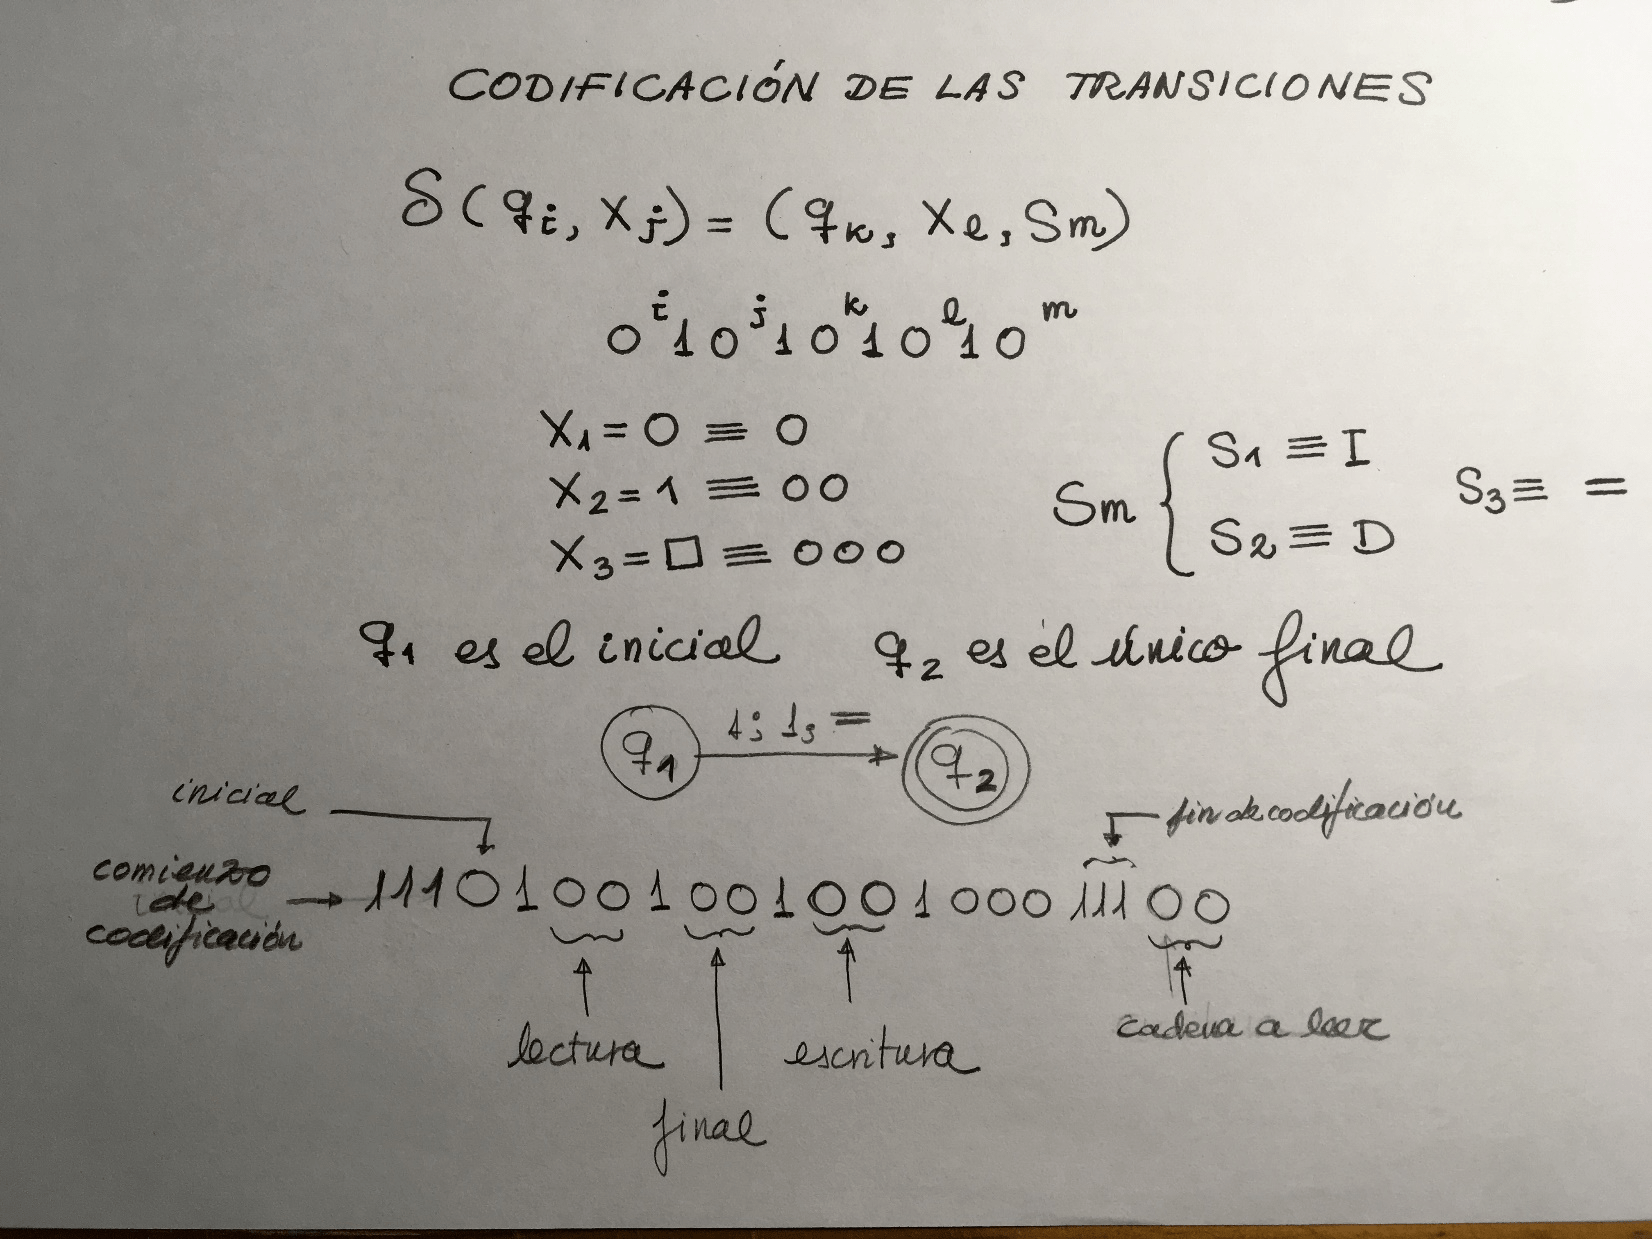
\includegraphics[scale=.2]{cod-mtnd.png}}
\end{figure}

\subsection{Salidas de la Máquina de Turing}
Dada una MT y una entrada, se pueden dar tres tipos de salidas:
\begin{itemize}
    \item La MT se detiene, y acepta la entrada (la palabra)
    \item La MT se detiene, y rechaza la entrada (la palabra)
    \item No se detiene
\end{itemize}

Dependiendo cuáles se den:
\begin{itemize}
    \item T-D: Se detiene con $a \in L$ en un estado final (acepta) y con $a \notin L$ en un estado no final (rechaza).
    \item T-R: Se detiene para $a \in L$ en un estado final, acepta todas las que pertenecen. Es menos restrictivo.
\end{itemize}

\section{Decidibilidad}
Un conjunto S se dice que es infinito contable si tiene la misma cardinalidad que $\mathbb{N}$ ($|S|=|\mathbb{N}|$) Si puede establecerse una correspondencia biyectiva entre los elementos de $\mathbb{N}$ y los elementos de S. Se puede decir este elemento es el primero, este el segundo, etc.

Un conjunto se dice que es contable si es finito o infinito contable.

Un conjunto no contable se dice que es incontable.

\subsection{Nociones formales}
$\aleph_0 < \aleph_1 \leq 2^{\aleph_0}$
\begin{itemize}
    \item Cardinalidad de los naturales: $\aleph_0$
    \item Cardinalidad de los enteros: $\aleph_0$
    \item Cardinalidad de los racionales: $\aleph_0$
    \item Cardinalidad de los reales: $2^{\aleph_0}$
\end{itemize}

Teorema: El conjunto de cadenas binarias infinitas es incontable.

\subsubsection{Biyección entre $\mathbb{N}\textit{ y }\mathbb{Q}^+$}
Poniendo todas las fracciones fijando primero denominador 1, 2, 3, ... para cada una de estas se ponen los numeradores 1, 2, 3, ... 

Se va recorriendo y contando siguiendo las diagonales, saltándose los que tengan un valor equivalente a uno ya contado. En el borde izquierdo se baja y se va subiendo en diagonal, una vez arriba se pasa a la derecha y se baja en diagonal.

Por lo que tienen la misma cardinalidad, se pueden numerar aunque sea paradójica.

\subsubsection{Biyección entre $\mathbb{N}\textit{ y }\mathbb{Z}$}
George Cantor lo demuestra. Se cuentan haciendo pasos de valor 1, el positivo y después el negativo. 

1 -1 2 -2 3 -3 4 -4 5 -5 ...

\subsubsection{Biyección entre $\mathbb{N}\textit{ y }\mathbb{R}$}
Teorema: No se puede. El conjunto de los números reales en [0,1) es incontable, y por ende, el de los números reales.

Se pueden listar los valores 0,... y cogiendo la diagonal de los decimales, si se le suma 1 con módulo 10 no se encuentra ese valor en los previos, por lo que habrá más.

\subsection{Máquina de Turing Universal}
Es aquella Máquina de Turing que recibe como cadena una descripción de lenguaje (M) y la cadena de entrada (w).

Es capaz de simular cualquier otra máquina de Turing.
\begin{itemize}
    \item Si M acepta w, U se parará en un estado final.
    \item Si M NO acepta w, U no se parará o bien se parará en un estado no final.
    \item Si M no se para, U tampoco.
\end{itemize}

\subsection{Algunos teoremas importantes}
Lenguaje Universal: $A_{MT}$ o $L_U$.

El complementario de un lenguaje está formado por aquellos elementos de $\Sigma^*$ que no están en L.
\begin{itemize}
    \item $L=\{x/|x|=2 \textit{ y x comienza con 1}\}$. $L=\{10,11\}$ y $\overline{L}=\{\lambda, 0, 1, 01, 000, ... \}$
\end{itemize}

\subsubsection{Teorema Hay lenguajes que no son reconocibles (NTR) por MTs}
$\exists L / L$ no es reconocible por una MT.

Si M no sabe decir (entra en bucle) si $w \in L$ entonces NTR.

El conjunto de todas las MT es contable, dado que $\Sigma^*$ es contable y se puede codificar una MT. 

Sea L el conjunto de todos los lenguajes del alfabeto de cadenas infinitas, se ha visto que es incontable.

Por lo tanto, algunos lenguajes no pueden ser reconocidos por MTs. Son NTR.

\subsubsection{Teorema $A_{MT}$ es Turing-reconocible}
Sea $A_{MT}=\{<M,w> | M \textit{ acepta }w\}$

La MT U simula M con entrada w. Es decir: U acepta o rechaza si M lo hace, y entra en bucle infinito si este lo hace.

\subsubsection{Teorema $A_{MT}$ es indecidible}
Se puede demostrar por reducción al absurdo.

Se construye H que decide $A_{MT}$, entonces construimos D, como H negada. Por último, pasamos como entrada la propia máquina D ($<D, <D>>$). Entonces llegamos al absurdo.

\subsubsection{Teorema $\overline{A_{MT}}$ es no-Turing-reconocible}
Teorema: Un lenguaje es decidible si y solo si es Turing-Reconocible y su complementario es también Turing-Reconocible.

L es TD $\Rightarrow$ L es TR y $\overline{L}$ es TR.

$\overline{A_{MT}}$ es el conjunto de $<M,w>$ que no reconocen w.

Sea $\overline{A_{MT}}$ Turing-reconocible. Entonces $A_{MT}$ seria Turing-decidible ($A_{MT}$ es TR), pero sabemos que es indecidible y, por tanto, $\overline{A_{MT}}$ es no-Turing-reconocible.

Otro lenguaje no-Turing-Reconocible es $EQ_{MT}=\{<M_1, M_2> | M_1, M_2 \textit{ son MTs y } L(M_1)=L(M_2)\}$, dadas dos MTs decide si son equivalentes (mismo lenguaje).

\subsubsection{Teorema $HALT_{MT}$ es indecidible}
Dada una MT universal, U, y su entrada $<M,w>$. Decide si M se para o no.

$HALT_{MT}=\{<M,w> / M \textit{ se para con w}\}$. Por absurdo se puede demostrar que no existe.
\begin{itemize}
    \item Construimos $H_1$, que niega la salida de H.
    \item Hacemos que $H_1$ sea la entrada de $H_1$. 
    \item Si H decide que $H_1$ se para, $H_1$ dice que no se para.
    \item Si H decide que $H_1$ no se para, $H_1$ dice que se para.
\end{itemize}

Alan Turing en 1936 demuestra que NO existe un algoritmo que resuelva este problema.

\subsection{Lenguaje Diagonal}
Se hace una matriz de M x w, Máquina de Turing y entrada.

Esta se completa de manera que: 
\begin{itemize}
    \item $(i, j)= 1 \Rightarrow w_i \in L(M_j)$
    \item $(i, j)= 0 \Rightarrow w_i \notin L(M_j)$
\end{itemize}  

$L_d = \{ w_i / M_i \textit{ no acepta } w_i\}= \{w_i / w_i \notin L(M_i)\}$

Sea $M_j$ la MT que acepta $L_d$ ($L_d = L(M_j)$):
\begin{itemize}
    \item $w_j \in L_d \Leftrightarrow (j,j)=0 \Rightarrow w_j \notin L(M_j)$
    \item $w_j \notin L_d \Leftrightarrow (j,j)=1 \Rightarrow w_j \in L(M_j)$
\end{itemize}

Es contradictorio.

\subsection{Resumen}
\begin{itemize}
    \item $A_{MT}$ o $L_U$ es Turing-Reconocible, pero no Turing-Decidible.
    \item $\overline{A_{MT}}$ o $\overline{L_U}$ es No-Turing-Reconocible.
    \item $HALT_{MT}$ es Turing-Reconocible.
    \item $L_d$ es No-Turing-Reconocible.
\end{itemize}

\subsection{Reducción de un problema A a otro problema B}
Reducir A a B es A en B, de modo que una solución a B pueda usarse para resolver A.

Si A se reduce a B (A es reducible a B), resolver A no será más difícil que resolver B.

$A \leq_m B$ mapping; $A \leq_p B$ polinomial time.
\begin{itemize}
    \item Que sea polinomial implica que la reducción se lleva a cabo una función cuyo $T(n)= O(n^k)$
\end{itemize}

Dados dos lenguajes A y B, y una función $f:\Sigma^* \rightarrow \Sigma^*$, f es una transformación del lenguaje universal del problema A al lenguaje universal del problema B.

$\forall w\in A \Leftrightarrow f(w)\in B$; $ A \leq_f B$

Teoremas:
\begin{enumerate}
    \item B decidible $\Rightarrow$ A decidible
    \item B Turing-reconocible $\Rightarrow$ A Turing-reconocible
    \item A no-Turing-reconocible $\Rightarrow$ B no-Turing-reconocible
    \item A indecidible $\Rightarrow$ B indecidible
    \item B decidible $\Rightarrow$ es fácil de resolver A es fácil
\end{enumerate}

Para probar que un problema B es indecidible bastará mostrar que un problema indecidible A se reduce a B.
\begin{itemize}
    \item Si A es difícil $\Rightarrow$ B es difícil
    \item Si B es difícil no podemos extraer conclusiones de A
    \item Si $A \leq_p B$ y $B \leq_p A$ entonces son igual de difíciles.
\end{itemize}

Ejem. 
\begin{itemize}
    \item El problema M de multiplicar dos números enteros y el problema C de elevar al cuadrado un número entero. El problema C es más fácil que el problema M. De hecho, si podemos hacer la multiplicación, se puede elevar al cuadrado un número multiplicándolo por sí mismo, por lo que $C \leq M$. $x \rightarrow (x,x)$
    \item $\textit{camino Hamiltoniano} \leq_p \textit{ciclo Hamiltoniano}$. Dado que para que sea ciclo tiene que ser primero camino. Por lo tanto, las soluciones a ciclo sirven a camino.
\end{itemize} 

\subsubsection{$HALT_{MT}$ es indecidible}
$A_{MT} \leq_m HALT_{MT}$
\begin{itemize}
    \item Construimos S para decidir $A_{MT}$
    \item Dentro R decide $HALT_{MT}$ y tenemos también M que es la MT de entrada. 
    \begin{itemize}
        \item Si M se para, S simula M con w hasta que pare.
        \begin{itemize}
            \item Si M acepta, S acepta.
            \item Si M rechaza, S rechaza.
        \end{itemize}
        \item Si M no se para, R rechaza, por lo que S rechaza.
    \end{itemize}  
\end{itemize}

Si R decide $HALT_{MT}$, S decide $A_{MT}$. Es decir, $A_{MT}$ se reduce a $HALT_{MT}$, pero $A_{MT}$ es indecidible (TR), luego $HALT_{MT}$ es indecidible (es TR, pero no TD).